\chapter{Vorlesung}
\section{AVL-Bäume von Adelson-Velsky and Landis}
\begin{wrapfigure}[2]{l}{0.3\linewidth}
	\vspace{-50pt}
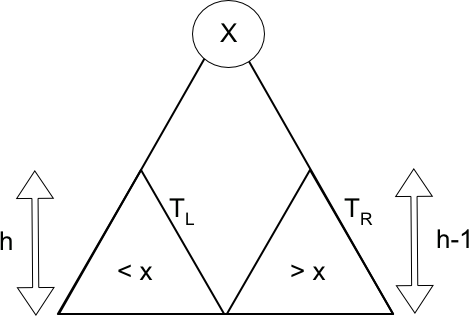
\includegraphics[width=\linewidth]{11/Grafik/img1.png}
\caption{}
\end{wrapfigure}

\vspace{30pt}
\paragraph{Ziel:}%
Zeige, dass die maximale Tiefe eines AVL-Baums mit n Knoten ($\hat{=}~ n$ gespeicherten Schlüsseln) $O(\log(n))$ beträgt.
\vspace{50pt}
\subsection{AVL-Eigenschaft:} 
$|h(T_L)-h(T_R)| \leq 1$ muss für jeden Knoten des Baums gelten. $~~~\Rightarrow$ Suchzeit $O(\log(n))$ im worst-case.\\
\begin{wrapfigure}{l}{0.3\linewidth}
	\vspace{40pt}
	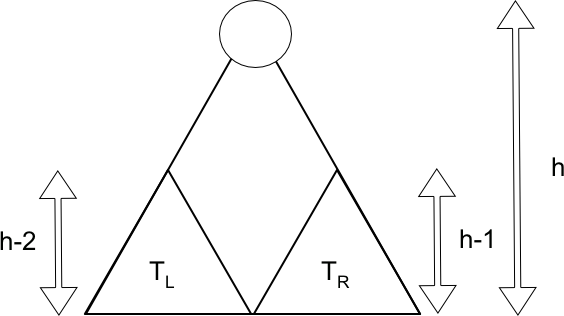
\includegraphics[width=\linewidth]{11/Grafik/img2.png}
	\caption{}
	\vspace{500pt}
\end{wrapfigure}

$n(h) =$ minimale Anzahl von Knoten in AVL-Baum der Tiefe h
\[n(h) \geq 1+n(h-2) + n(h-1)\text{ mit  }n(0)=0\text{ und }n(1)=1\]
\[n \geq f(h)\footnote{$f(h)$ meint hierbei die h-te Fibonacci-Zahl} = \frac{1}{\sqrt{5}} \cdot (\phi^h-\phi^{-h})\text{ mit}\] 
\[\phi = \frac{1+\sqrt{5}}{2} \approx 1,61\ldots\]
\[\Rightarrow n \geq c \cdot \phi^h\]
\[\Leftrightarrow h \leq \log{(\frac{n}{c})}\]
\[\Rightarrow h \in O(\log{n})\]
\begin{flushright}
	q.e.d.
\end{flushright}
\clearpage

\section{Rotationen}

\begin{figure}[H]
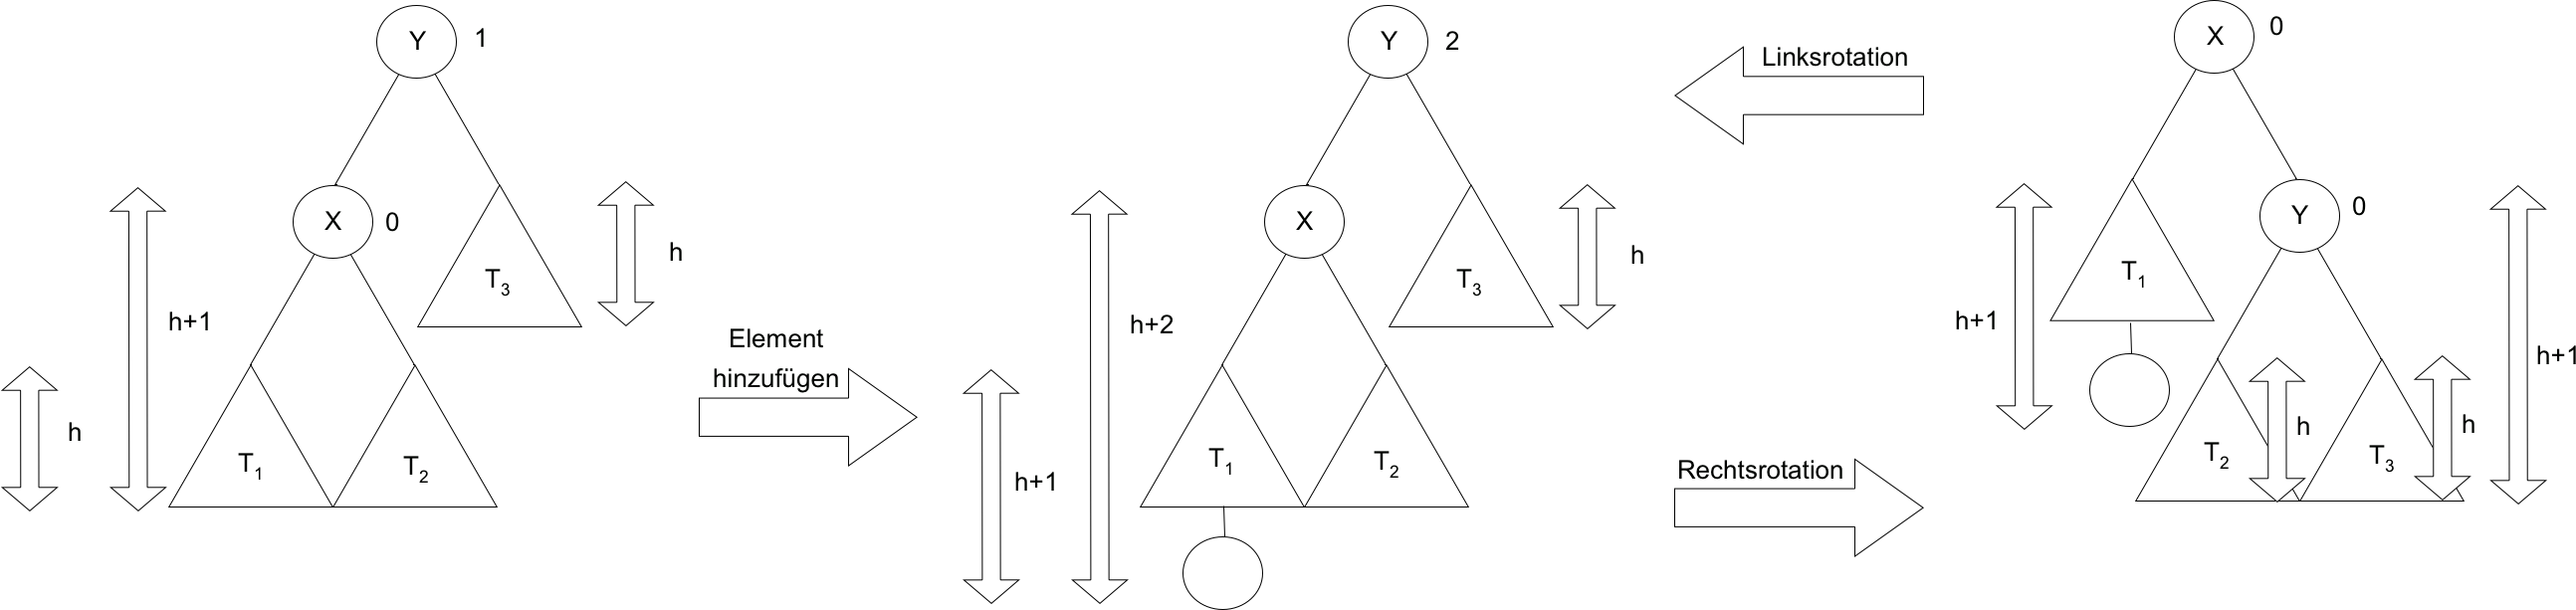
\includegraphics[width=\textwidth,left]{11/Grafik/img3_Rotation.png}
$Keys(T_1) < Key(X) < Keys(T_2) < Key(Y) < Keys(T_3)$ \\
\lstinline[language=Java]{balance(Y) = height(Y.left)-height(Y.right)}
\end{figure}

\begin{wrapfigure}{l}[-18pt]{0.24\textwidth}
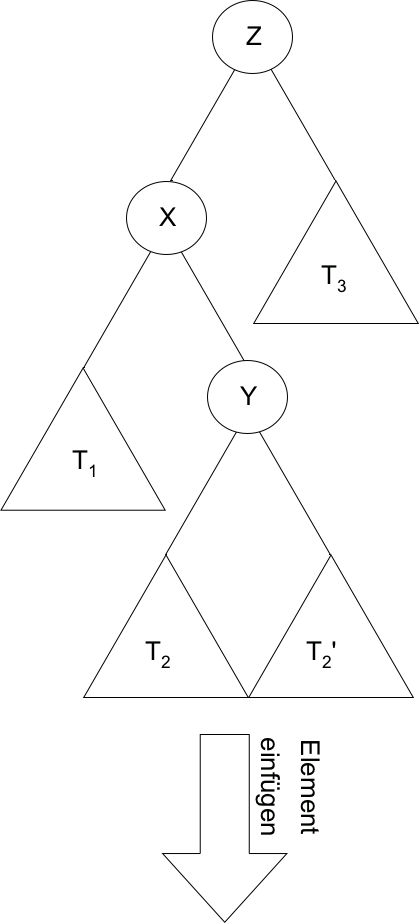
\includegraphics[width=0.9\linewidth]{11/Grafik/img4_doppelRotation_1.png}
\end{wrapfigure}

$Keys(T_1) < Key(X) < Keys(T_2) < Key(Y) < Keys(T_2^{'}) < Key(Z) < Keys(T_3)$

\begin{figure}
	\vspace*{-40pt}
	\begin{subfigure}[H]{0.3\textwidth}
		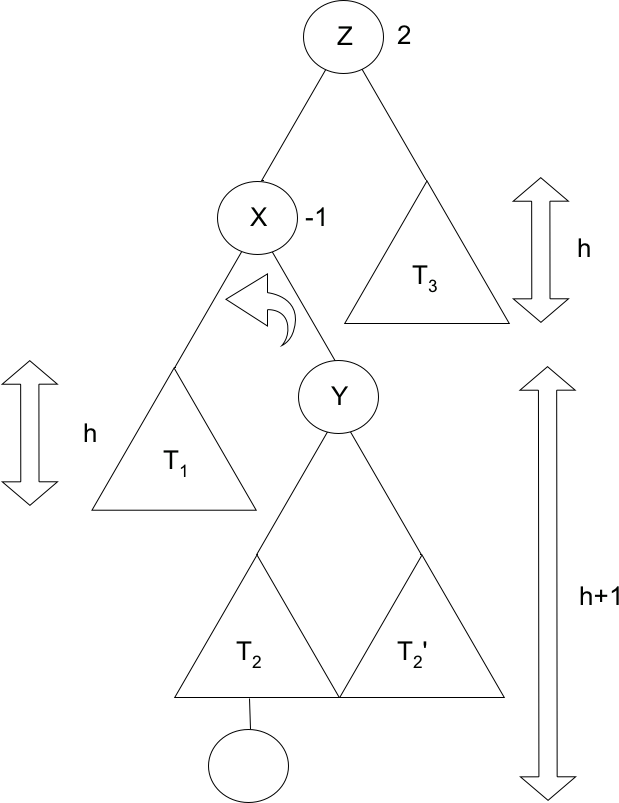
\includegraphics[width=\linewidth]{11/Grafik/img5_doppelRotation_2.png}
	\end{subfigure}
	\begin{subfigure}[H]{0.3\textwidth}
			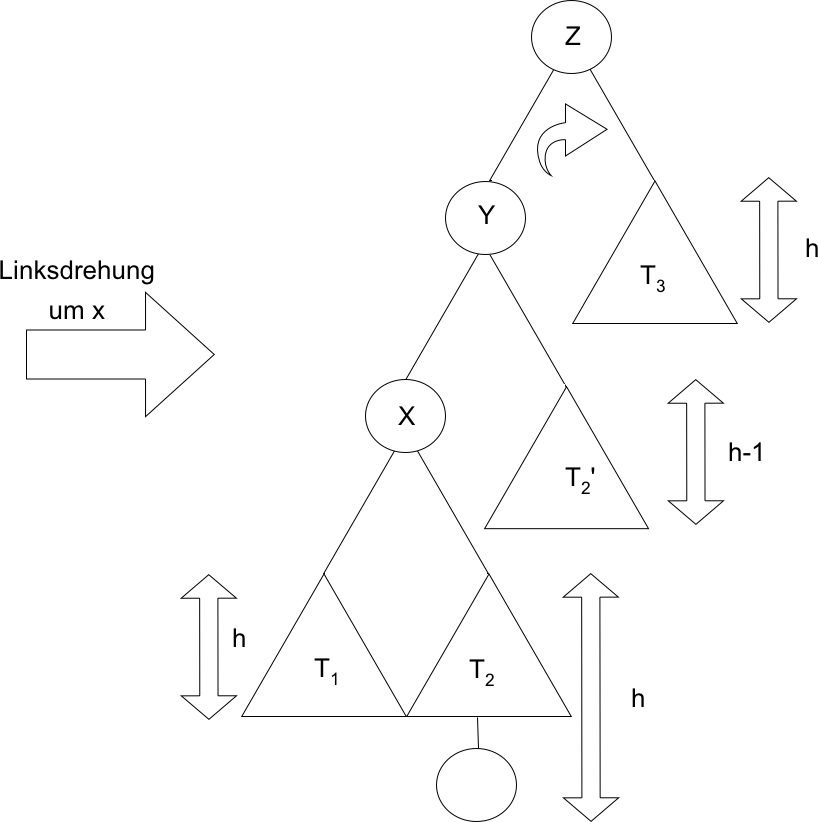
\includegraphics[width=\linewidth]{11/Grafik/img6_doppelRotation_3.png}
	\end{subfigure}
	\begin{subfigure}[H]{0.4\textwidth}
				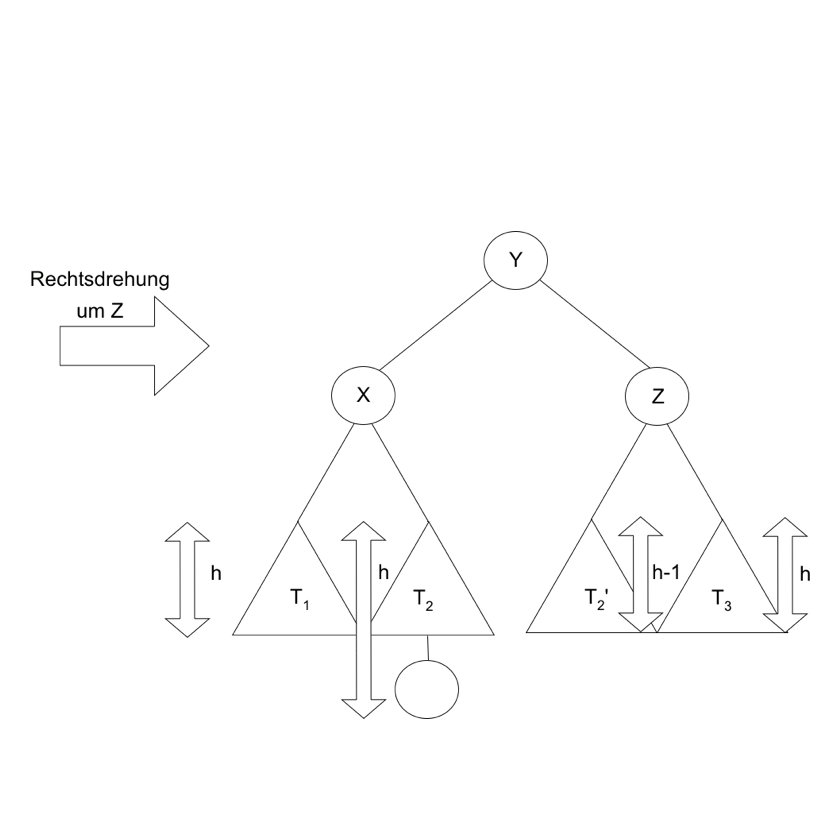
\includegraphics[width=\linewidth]{11/Grafik/img7_doppelRotation_4.png}
	\end{subfigure}
	\caption{Rotationen}
\end{figure}

%\clearpage
\newpage


\section{Pseudo-Code}
\lstinputlisting[language=Java, style = pseudo]{11/Code/Node.java}

\paragraph{Anmerkung:} Die Laufzeit des Einfügens bleibt in $O($Baumtiefe$)$ = $O(\log{n})$. Nur einer der vier Fälle ist notwendig, um die Balance herzustellen. 
\pagebreak